\chapter{Testing}


\section{Unit tests}
\subsection{Description of the tests}
    \begin{itemize}[noitemsep]
        \item Question Service
            \begin{itemize}[noitemsep]
                \item GetQuestion(testType): gets the question
                \item GetQuestion(testType): throws a business exception as the question does not exist
                \item GetQuestions(testType): gets the questions correctly
                \item AddQuestions(testType): adds a new question
                \item UpdateQuestion(testType): does not throw an exception
            \end{itemize}
        \item User Service
            \begin{itemize}[noitemsep]
                \item GetUser(): gets the user correctly
                \item GetUserByEmail(email): gets the user correctly
                \item ChangePassword(email, password, newPassword): changes the password
                \item ChangePassword(email, password, newPassword): throws a business exception when the token is not valid anymore
                \item ChangePassword(email): throw a business exception as the user does not exist
                \item AddUser(email, password): returns the guid correctly
                \item AddUser(email, password): throw a business exception as the user already exists
                \item UpdateTokenPasswordRecover(email, token): updates the token correctly
                \item UpdateTokenPasswordRecovery(email, token): throw a business exception when the user does not exist
                \item ChangeEmail(email, newEmail): changes the email correctly
                \item ChangeEmail(): throw a business exception when the user does not exist 
                \item ChangeEmail(email): throw a business exception when the user is already in use
                \item UpdateTokenEmailConfirmation(email, token): updates the token correctly
                \item UpdateTokenEmailConfirmation(email, token): throws a business exception when the email has already been confirmed
                \item CheckConfirmedUser(email): throw a business exception when the user does not exist
                \item ConfirmEmail(email): confirms the email correctly
                \item ConfirmEmail(email): throws a business exception when the user does not exist
                \item ConfirmEmail(email): throws a business exception when the token is not valid anymore
                \item UpdateTokenEmailConfirmation(email, token): throws a business exception when the user does not exist
                \item CheckConfirmedUser(email): confirms correctly
                \item DeleteUser(email): deletes the user correctly
                \item DeleteUser(email): throws a business exception when the user does not exist
            \end{itemize}
        \item TestService
            \begin{itemize}[noitemsep]
                \item DeleteTest(): deletes the test 
                \item AddTest(): returns the guid 
                \item GetTest(): gets the test correctly
                \item GetAll(): gets all the tests correclty 
                \item DeleteTest(): throws a business exception when the test does not exist 
                \item DeleteAllTestsFromUser(): deletes all the tests correctly
            \end{itemize}
        \item Extensions
            \begin{itemize}
                \item FilterTests(): filters correctly
            \end{itemize}
    \end{itemize}

I created a unit testing project for the backend, as I wanted to test all parts in the application that used business logic. 
This way, I could change the implementation in the future but all requirements would keep intact, as I would notice if it is not done according to the correct logic. 

The coverage of the testing unit is small, due to the fact that I don't use unit testing for the controllers, simple entities and implementations for 
third-party libraries nor configurations. I only use unit testing when it really helps me. 

Thanks to report tools, such as \textit{dotnet-test} and \textit{dotnet-reportgenerator} \cite{Coverage} I created this review.

\begin{figure}[H]
    \centering
        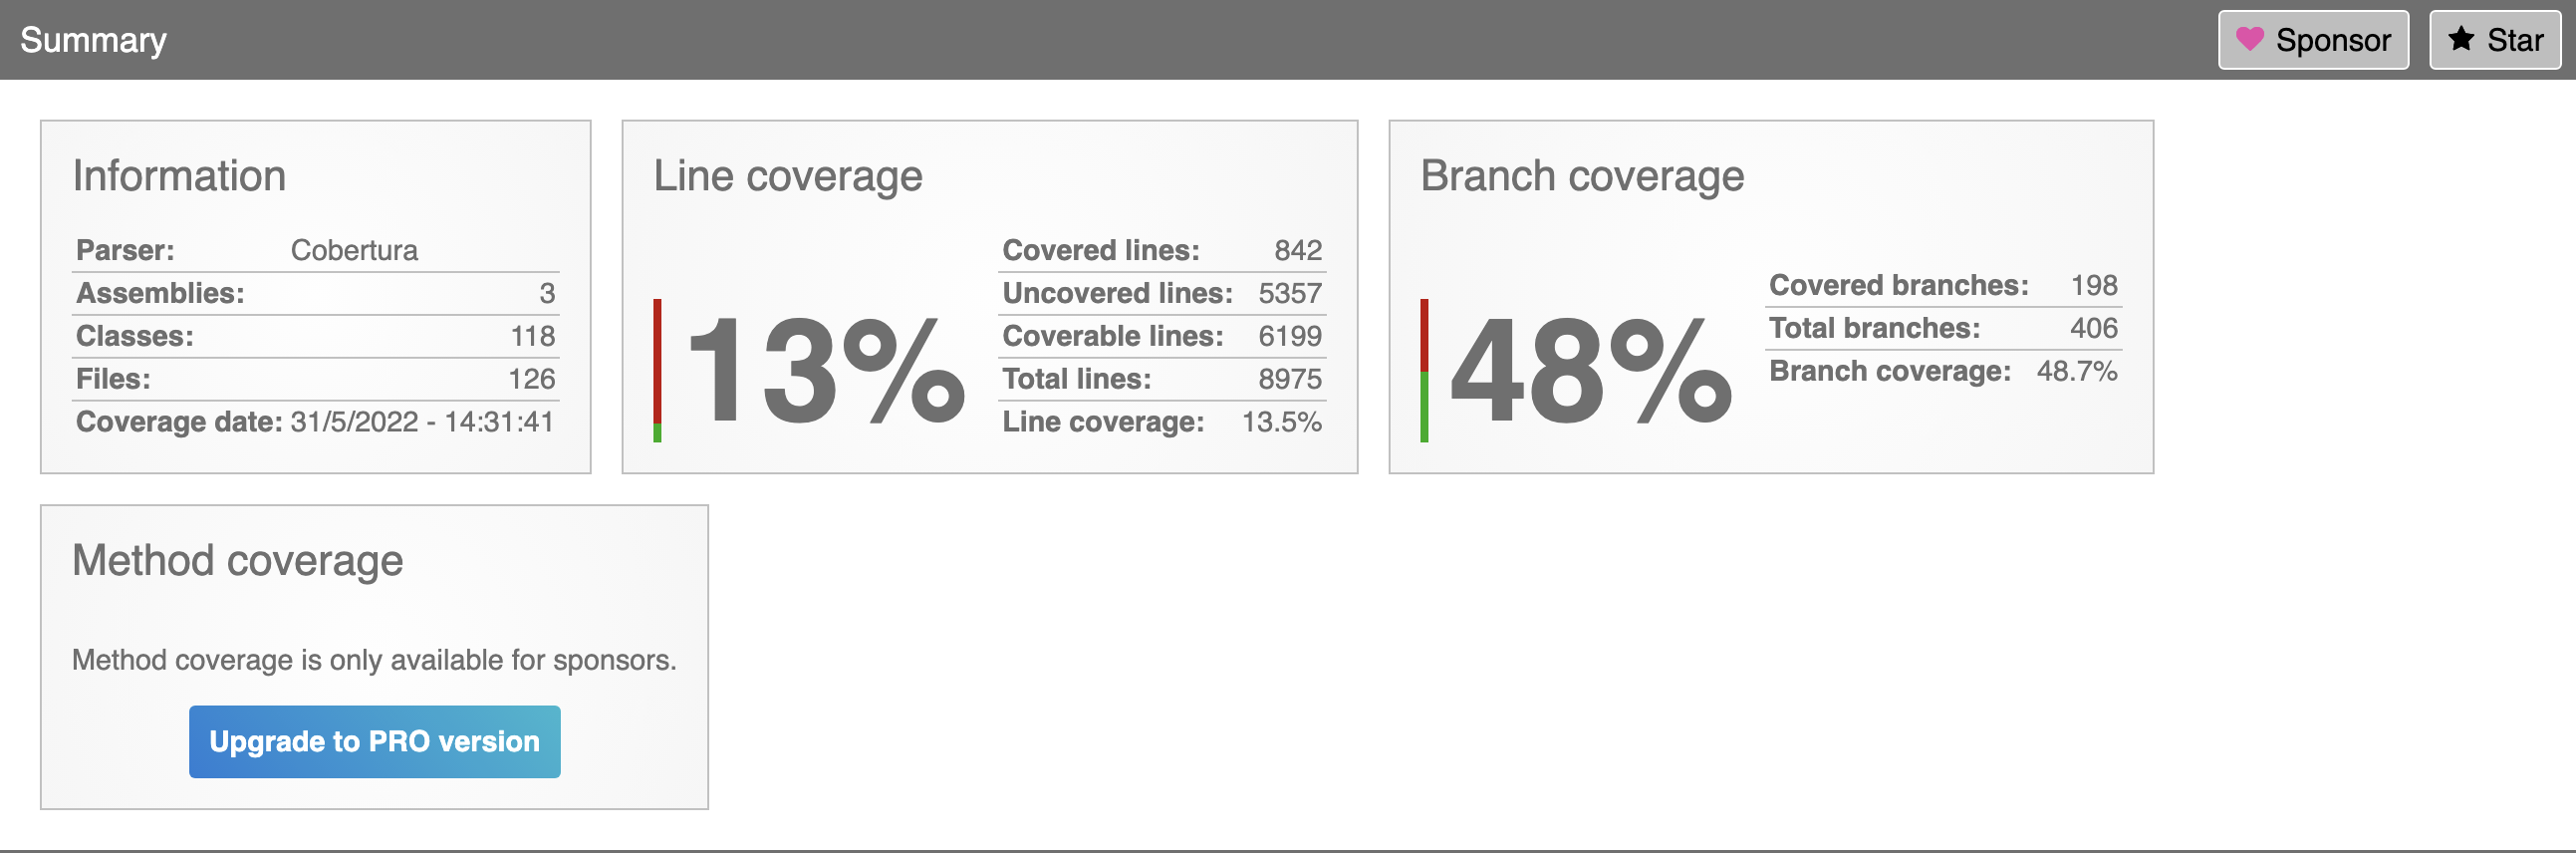
\includegraphics[width=\textwidth]{assets/coverage.png}
    \caption{Test coverage}
    \label{fig:test_coverage}
\end{figure}

The following figure shows the fragments of code that have a higher complicity, to be refactored or tested more exhaustively. 
It is measured using \textbf{cyclomatic complexity}, which counts the number of alternative flows that a program/function could have.
\begin{figure}[H]
    \centering
        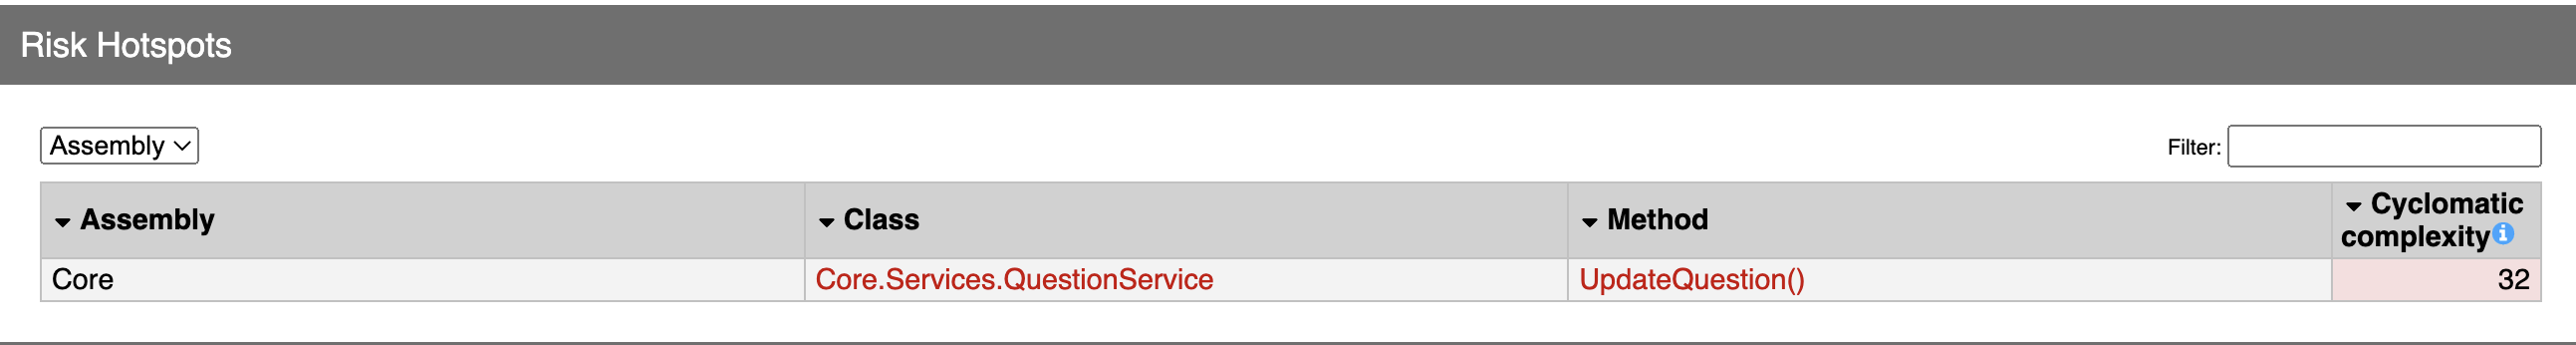
\includegraphics[width=\textwidth]{assets/risk_hotpots.png}
    \caption{Risk hotspots}
    \label{fig:test_hotspots}
\end{figure}

A more in-detail figure \ref{fig:test_coverage_detail} about the test coverage of the backend project. It shows how the core part of the application and the repositories are the most 
tested features of the application. The use of third party libraries will be better tested using other tools later on.
\begin{figure}[H]
    \centering
        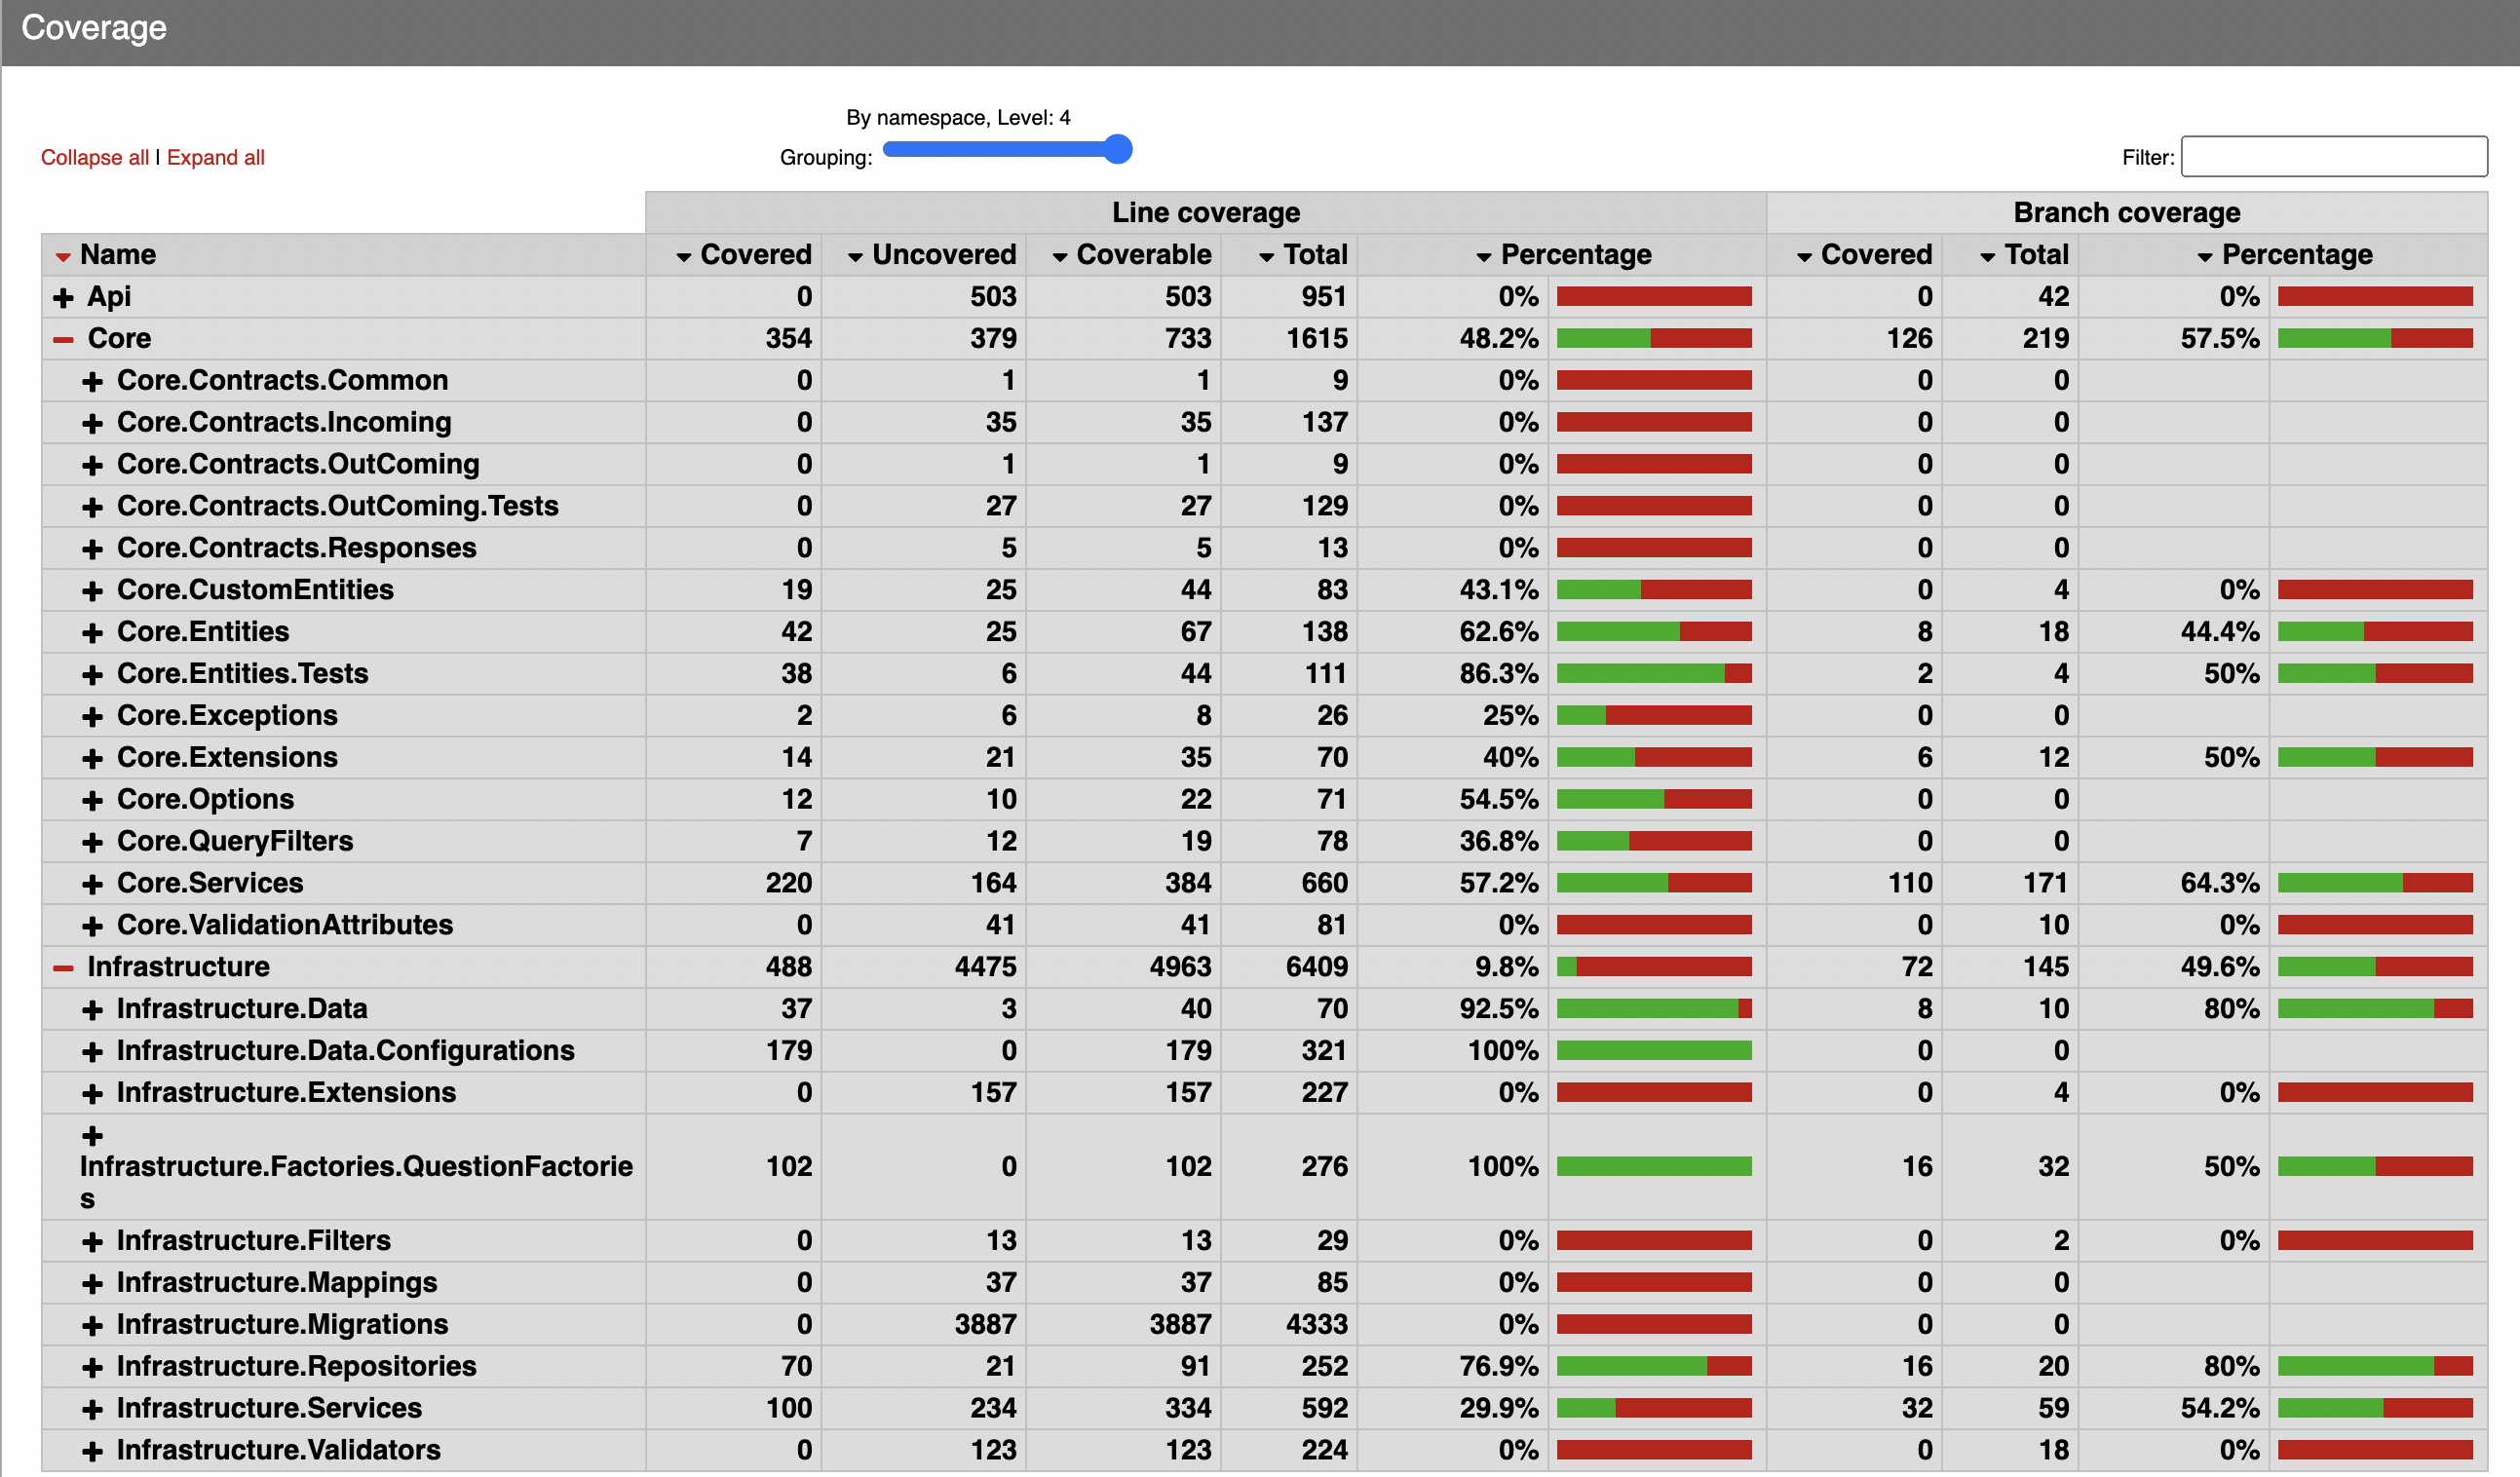
\includegraphics[width=\textwidth]{assets/coverage_detail.png}
    \caption{Coverage in detail}
    \label{fig:test_coverage_detail}
\end{figure}

\subsubsection{Implementation}
    As I should separate the environments as much as possible, the databases should be different too. For testing purposes, I use an in-memory database, so I don't 
    create a real database and the queries are faster. 
    The database context is then mocked (see figure \ref{lst:test_mock_unit_work}).

    \lstinputlisting[language=CSharp, captionpos=t,
                caption={Mocking the Unit of Work}, 
                label={lst:test_mock_unit_work}]
    {code/MockUnitOfWork.cs}

\paragraph{Test structure} it follows the \textbf{AAA} schema (\textit{Arrange, Act, Assert}). 
    The first \textit{A}, \textit{Arrange} is for setting up, initializing and configuring all the neccessary objects for the test to work. 
    The second one, \textit{Act} is where the actions to be tested is done. 
    The last one, \textit{Assert} is where the actions are tested. \textit{See figure \ref{lst:test_aaa}.}
    \lstinputlisting[language=CSharp, captionpos=t,
        caption={Test structure: AAA}, 
        label={lst:test_aaa}]
    {code/TestStructure.cs}

\paragraph{Arguments:} the tests can receive or not arguments. If I use the \textit{Fact} attribute, it means that the test does not need any argument. 
    It could be because the functions inside the test don't need any argument, I just need to test an use case or the arguments are not important. 
    If I use \textit{InlineData}, the arguments of the attribute will be passed to the function. This works fine when I just need to pass an use case or, although the arguments are irrelevant I don't want to use 
    them in the code as \textit{magic numbers or words}. 
    \textit{MemberData} allows to pass as argument a field of the class or a method. I use them when I need to test the method in multiple use cases. This way, I can have in a field or function a list of all use cases that I need to test. 
    The function \textit{AllTestTypes} (see figure \ref{lst:test_arguments}) shows how to use all the types from an \textit{Enum} as use cases.
    \lstinputlisting[language=CSharp, captionpos=t,
        caption={Test arguments}, 
        label={lst:test_arguments}]
    {code/TestArguments.cs}

\section{Integration tests}
I use \textbf{Postman} to test the API calls. It uses \textbf{Chai Assertion Library} \cite{Chai} for its tests and have a new feature which is actually in \textit{Beta}, called \textbf{Postman flows}. 

\subsection{API tests}
Firstly, I created a collection using the JSON file created from \textit{Swagger} due to my API documentation is made using \textit{OpenApi}. 
In this collection \ref{fig:test_collection}, all calls to the API are defined. Also, there are environment variables to avoid using \textit{magic values} or to change them using the tests. We'll see it later.
\begin{figure}[H]
    \centering
        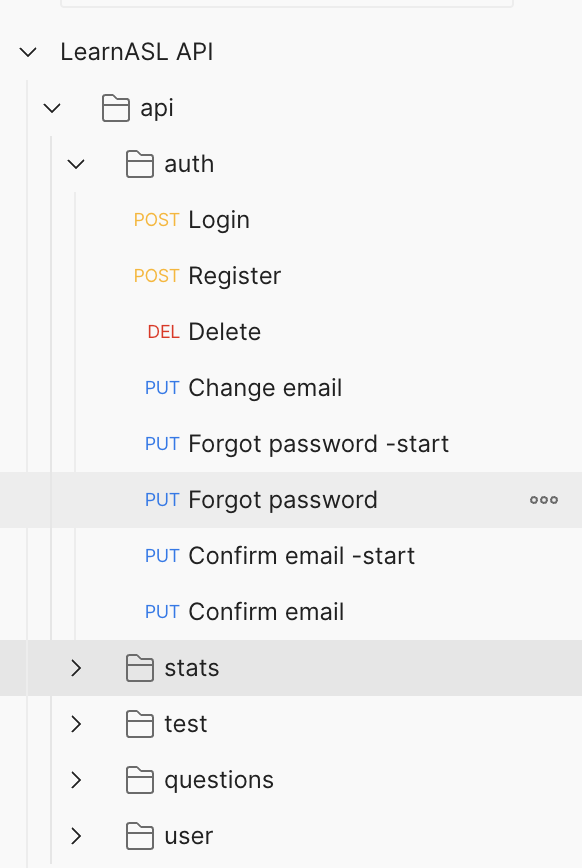
\includegraphics[width=0.5\textwidth]{assets/postman_collection.png}
    \caption{Postman collection}
    \label{fig:test_collection}
\end{figure}

This way, to \textbf{define a call} I just set the HTTP verb, the route and define the parameters and auth headers. \textit{See figure \ref{fig:test_call}}.
\begin{figure}[H]
    \centering
        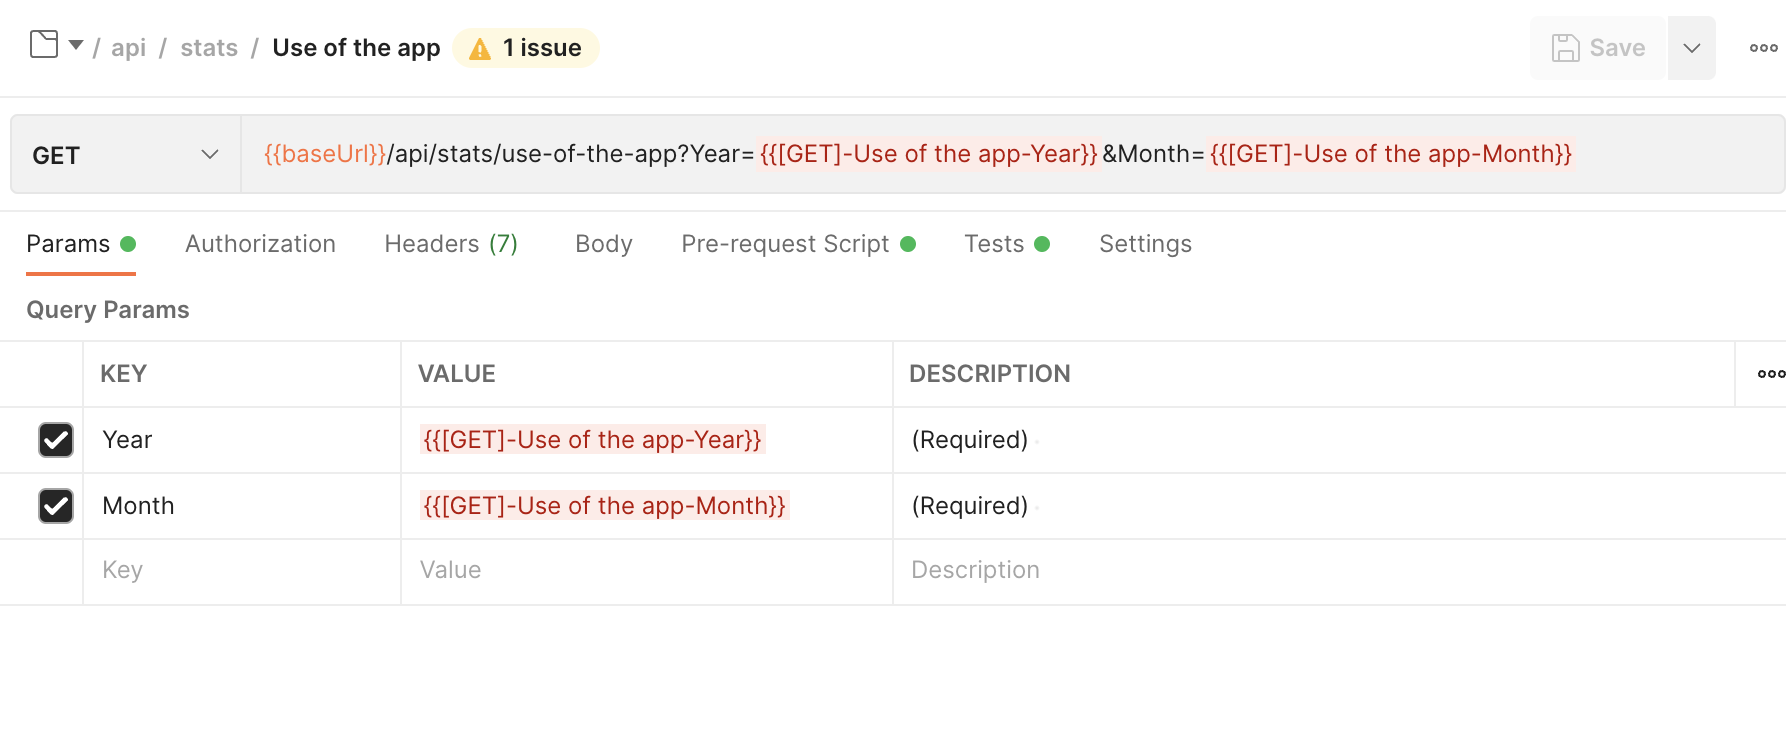
\includegraphics[width=\textwidth]{assets/postman_call.png}
    \caption{Postman call}
    \label{fig:test_call}
\end{figure}

\subsubsection{Testing a call}
A call can also have tests. This way, each time the call is made these tests are executed. These tests are executed after doing the call, so this is intercepted. 
There is also another environment, called \textbf{Pre-request}, which is executed before the request. This allows to set up the environment for the test and define some variables. 

To run the call with different parameters so that I can test different use cases, I have to define the use cases in the \textit{Pre-request} 
environment and execute the rest of the calls after the first one. 

In the next fragment of code \ref{lst:test_prerequest}, I define all use cases parameters for this call. Each use case has the arguments and the result expected. I set an environment variable for them.
\lstinputlisting[language=javascript, captionpos=t,
        caption={Pre request}, 
        label={lst:test_prerequest}]
{code/postman/prerequest.js}

In the next fragment of code \ref{lst:test_tests}, I show the \textit{Test environment}. As the evaluating process is done multiple times, 
I created a function to evaluate it. The first thing that I have to do is evaluating the current call, so that I test the last call. 
Then, I should test the rest of use cases. For this, I read the environment variable where I define the rest of use cases and iterate it. 
In each iteration I should create a new request. In every request, the \textit{Pre request} environment is executed. That is why I delete 
a use case from it. The last thing to do is cleaning the environment, so that these environment variables don't exist anymore.
\lstinputlisting[language=javascript, captionpos=t,
        caption={Testing environment}, 
        label={lst:test_tests}]
{code/postman/tests.js}

\subsubsection{Testing a flow}
This is a \textit{Beta} feature. As some calls depends on others, it could be interesting to concat them. 

For instance, almost every call depends on the auth flow. This way, I could chain the login call to the other one. 
Other example is deleting a test, because I should first create it.

\textit{Postman flows} allow me to chain the calls, execute all their tests and log the results. I created two use cases:
The next use case shows the flow to login in the application and get all the stats from the current user. When the logic call 
is executed, the environment variables are set to identify this user. Then, it is get from the stats calls to retrieve their stats. 
All tests are executed and the summary is logged. \textit{See figure \ref{fig:test_getstats}}.
\begin{figure}[H]
    \centering
        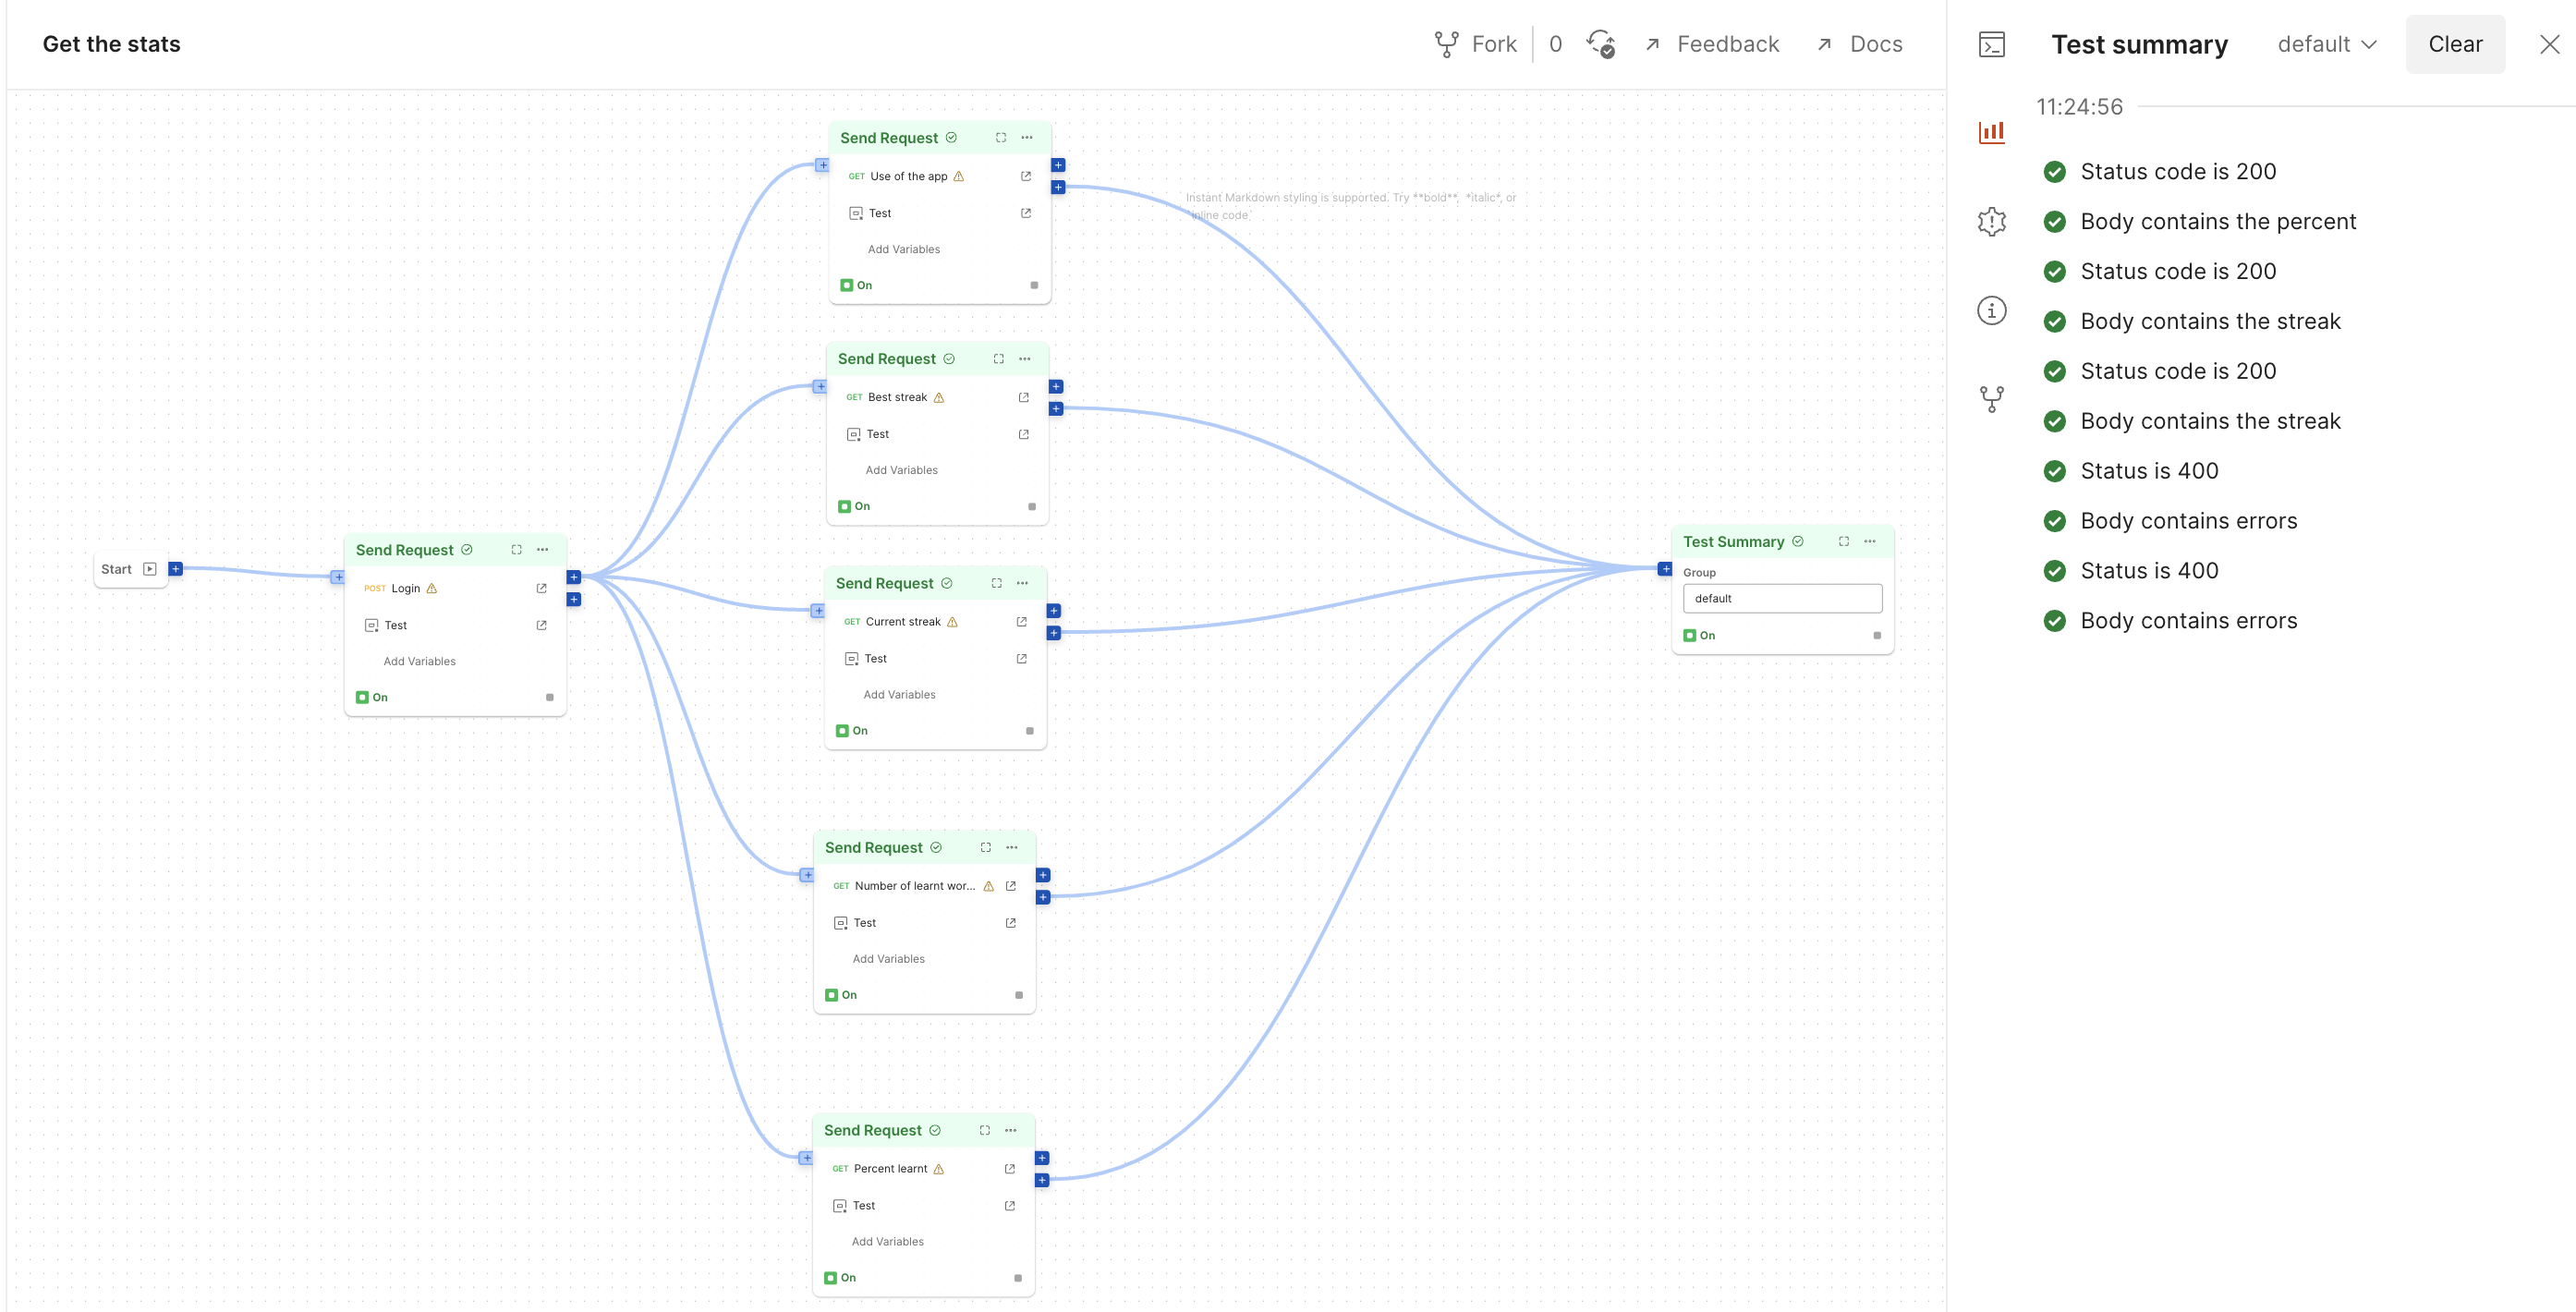
\includegraphics[angle=90, width=\textwidth, height=\textheight]{assets/postman_getstats.png}
    \caption{Use case: get the stats}
    \label{fig:test_getstats}
\end{figure}

The next use case \ref{fig:test_createanddeleteatest} shows the flow of a user that logins in the application, creating some tests and deleting one of them. 
This way, I chain the login request with the \textit{Create a test} request. The tests are executed and if the last call has a \textit{201} code, 
the next call can be executed, as the test has already been created and can be deleted. The environment is updated so that the id of the test to delete 
is the last created and this id is used for the deletion call.
\begin{figure}[H]
    \centering
        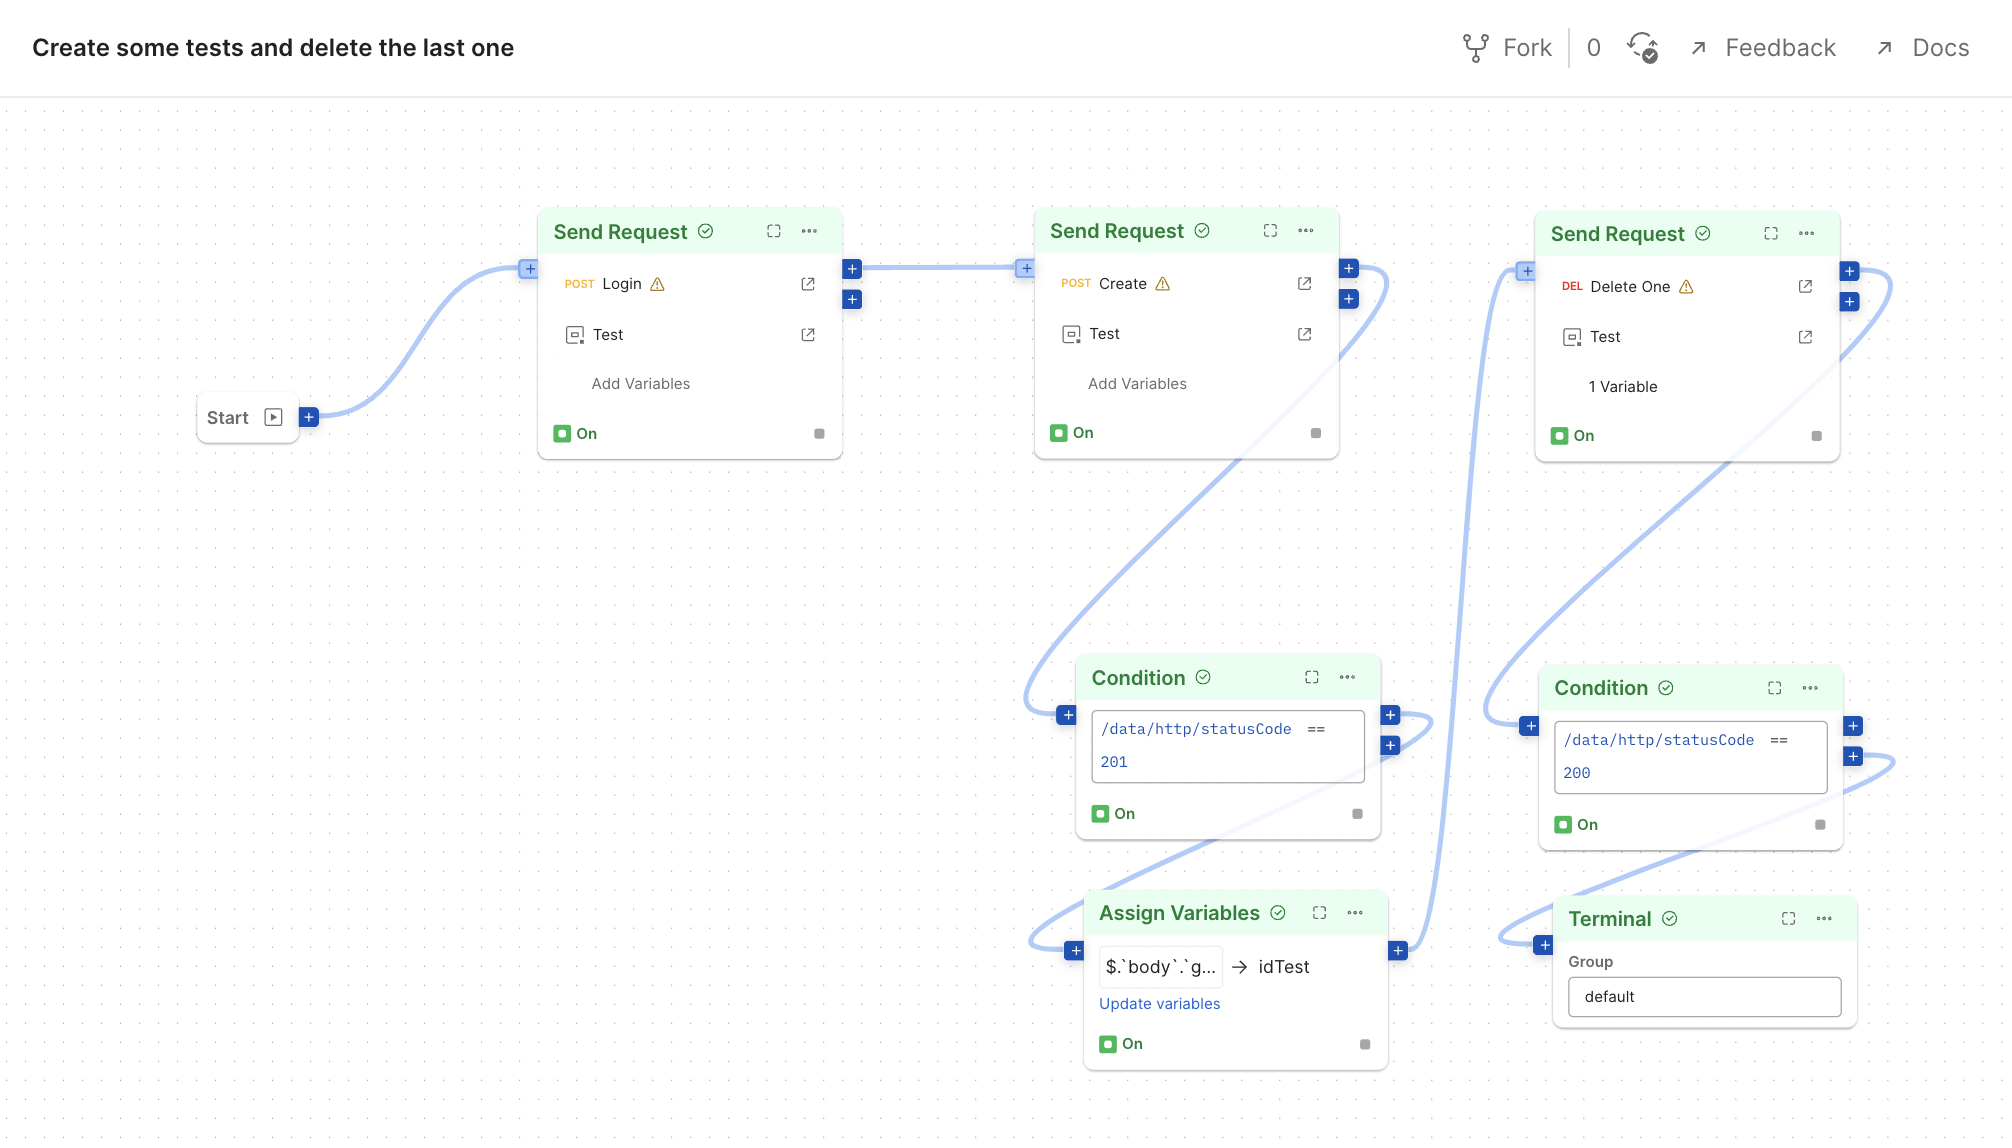
\includegraphics[angle=90, width=\textwidth, height=\textheight]{assets/postman_delete.png}
    \caption{Use cases: create some tests and delete the last one}
    \label{fig:test_createanddeleteatest}
\end{figure}

\section{Continious integration}
As I used \textit{GitHub} for the development and I created a new branch for every new feature, then did a pull request and merged all the changes, continious integration using \textbf{GitHub Actions} allowed me to 
automatically test my changes and see if I should merge or not. 

This way, I created a \textit{GitHub Action} \ref{lst:test_ga} that runs the tests for the backend each time a push or pull request that affects the \textit{backend} project is made in the repository.
\lstinputlisting[language=yaml, captionpos=t,
    caption={GitHub Action for continious integration}, 
    label={lst:test_ga}]
{code/backend.yml}